	\documentclass[12pt,a4paper,italian]{article}


\usepackage[italian]{babel}
\usepackage[latin1]{inputenc}
\usepackage{amsmath}
\usepackage{amsfonts}
\usepackage{amssymb}
\usepackage{color}
\usepackage{xcolor}
\usepackage{hyperref}
\usepackage[all]{hypcap}
\usepackage{ifthen}
\usepackage{wrapfig}
%\author{Piero Bizzotto}
\usepackage[top=2cm,bottom=5cm,left=80pt,right=80pt]{geometry}
\usepackage{graphicx}
\DeclareGraphicsExtensions{.jpg,.png}

\newcommand{\ajax}{AJAXDRAW}
\newcommand{\sito}{\href{http://ajaxdraw.sourceforge.net}{http://ajaxdraw.sourceforge.net}}

\setlength{\parindent}{0pt} %settato indentazione di default 
\setlength{\headheight}{3cm} %settato grandezza header...in altre parole, quanto distanzio il doc dall'intestazione

\usepackage{fancyhdr} %pacchetto per le intestazioni
\pagestyle{fancy} %uso del pacchetto


\fancyhead{} %annulla head di default
\fancyfoot{} %annulla foot di default


\usepackage{lastpage} %setto pg di pgtot a rfoot
     \rfoot{pagina \thepage\ di \pageref{LastPage}}


\lfoot{Versione: \insertversion} %setto versione doc a lfoot
\renewcommand{\footrulewidth}{0.5pt} %ridefinisco il valore della riga di intestazione
\renewcommand{\headrulewidth}{0.5pt} %ridefinisco il valore della riga di pie' di pagina

\newcommand{\insertversion}{0.0} %definisco il nuovo comando per inserire la versione


\lhead{  \begin{Huge} \ajax \end{Huge} \\  %intestazione di sinistra
					%\begin{Large}	Software per il Disegno Grafico\\ in Tecnologie Web \end{Large}  
					\begin{normalsize}\sito \end{normalsize}
			%\\ versione documento: \insertversion\ del \today} %setto l'intestazione sx
		}
\rhead{ %includo logo nell'intestazione dx
	 	
\includegraphics[scale=0.5]{../logo/logo.png}  
}


%CREAZIONE ELENCHI NUMERATI PERSONALIZZATI
\newcounter{Lcount}
\newcounter{Rcount}
\setcounter{Lcount}{0}
\setcounter{Rcount}{0}

\newenvironment{elenconumerato}[2][ ]
{
  \begin{list}{#1\arabic{Lcount}.}
    {
	\setcounter{Rcount}{\value{Lcount}}
	\setcounter{Lcount}{0} 
	\usecounter{Lcount} 
\addtolength{\leftmargin}{#2pt}
	}
}
{
  \end{list}
 \setcounter{Lcount}{\value{Rcount}}
}

%CREAZIONE ELENCHI PUNTATI
\newenvironment{elencopuntato}[1][]
{
\begin{list}{\textbullet} %\itemindent=#1pt
	{
	\addtolength{\leftmargin}{#1pt}
	}
} 
{
\end{list}
}


\newenvironment{elencodescrittivo}[1][]{\begin{description} \setlength{\itemindent}{#1pt} \addtolength{\leftmargin}{#1pt}} {\end{description}}

\newcommand{\TITOLODOC}{Titolo}

%footer centrale
\cfoot{ \TITOLODOC \\  E-mail:    \href{ mailto:webshape.contact@gmail.com}{ webshape.contact@gmail.com}  }

%INSERIMENTO IMMAGINI
\newcommand{\imagerealsize}[1]{\vspace{20pt} \includegraphics{#1} }
\newcommand{\imageadapted}[1]{\vspace{20pt} \includegraphics[width=1\textwidth]{#1} }

\newcommand{\glosspath}{.\glossario}
\newcommand{\gloss}[1]{\hyperref{\glosspath~\glossario.pdf}{}{#1}{#1}}

\hypersetup{
    %bookmarks=true,         % show bookmarks bar?
    %unicode=false,          % non-Latin characters in Acrobat’s bookmarks
	%pdftoolbar=true,        % show Acrobat’s toolbar?
	%pdfmenubar=true,        % show Acrobat’s menu?
    %pdffitwindow=true,      % page fit to window when opened
    %pdftitle={My title},    % title
    %pdfauthor={Author},     % author
    %pdfsubject={Subject},   % subject of the document
    %pdfnewwindow=true,      % links in new window
    %pdfkeywords={keywords}, % list of keywords
    colorlinks=true,         % false: boxed links; true: colored links
    linkcolor=black,           % color of internal links
    %citecolor=green,        % color of links to bibliography
    %filecolor=magenta,      % color of file links
    urlcolor=teal    % color of external links
%	linktocpage=false;
}


%COLORAZIONE TESTO
\newcommand{\blue}[1]{{\color {blue} #1}} 
\newcommand{\red}[1]{{\color {red} #1}}
\newcommand{\green}[1]{{\color {green} #1}}
\newcommand{\sezione}[1]{\leftskip=0pt \section{#1} \leftskip=18pt}
\newcommand{\subsezione}[1]{\leftskip=18pt \subsection{#1} \leftskip=36pt}
\newcommand{\subsubsezione}[1]{\leftskip=36pt \subsubsection{#1} \leftskip=54pt}
\newcommand{\subsubsecindent}{54}
\newcommand{\subsecindent}{36}
\newcommand{\secindent}{18}
\newcommand{\normindent}{8}
\newcommand{\code}[1]{{\bfseries \texttt{#1}}}
\newcommand{\paragrafo}[1]{\leftskip=36pt \paragraph{#1} \leftskip=54pt}
\newcommand{\subparagrafo}[1]{\leftskip=54pt \subparagraph{#1} \leftskip=72pt} %BASE!!!
\usepackage{multirow}
\title{\TITOLODOC}
\author{Dal Bosco Davide}

\begin{document}

\renewcommand{\insertversion}{1.0} %INSERIRE LA VERSIONE QUI DENTRO STILE x.x.xx
\renewcommand{\TITOLODOC}{Specifica Tecnica} %INSERIRE IL TITOLO DEL DOCUMENTO DA FAR COMPARIRE A PIE PAGINA
\renewcommand{\glosspath}{.\glossario} %INSERIRE PERCORSO RELATIVO

%%%%%%%%%%%%%%%%%%%%%%PARTE DA NON MODIFICARE%%%%%%%%%%%%%%%%%
\begin{titlepage}
\begin{center}
	\begin{Large}	\today \end{Large}
\end{center}

\vspace{20pt}

\begin{center}
	\begin{Huge}
				\textbf{\ajax}
	\end{Huge}
\end{center}			

\begin{center}
	\begin{large}
				\textbf{Software per il Disegno Grafico\\ in Tecnologie Web}
	\end{large}
\end{center}			

\vspace{20pt}

\begin{center}

\includegraphics[width=150pt]{../logo/logo}
\end{center}

\vspace{170pt}
\begin{center} %INSERIRE ALL'INTERNO IL TITOLO DOCUMENTO CHE COMPARIRA NELLA PAGINA INIZIALE				
	\begin{Huge}
				\textbf{\TITOLODOC}
	\end{Huge}
			\\
\end{center}
\vspace{190pt}
\begin{center}
Versione: \insertversion
\end{center}
\end{titlepage}

\newpage
%%%%%%%%%%%%%%%%%%%%%%FINE PARTE DA NON MODIFICARE%%%%%%%%%%%%%%%%%

\begin{center} %INSERIRE ALL'INTERNO IL TITOLO DOCUMENTO CHE COMPARIRA NELLA PAGINA INIZIALE
	\begin{Huge}	
				\textbf{\TITOLODOC}
			\\
	\end{Huge}
\end{center}

%\setlength{\parindent}{18pt} %settato indentazione di default 
\section*{\LARGE Sommario:}
Il presente documento descrive le scelte tecniche, architetturali e tecnologiche effettuate dall'azienda WebShape per lo sviluppo del Capitolato C04.

 %SEZIONE SOMMARIO
\indent \indent

\section*{\LARGE Stato del documento:}
\indent \indent
	Formale Esterno

\section*{\LARGE Redazione:}
	\begin{table}[!h]
		\begin{center}
			\begin{tabular}
				{|c|c|}
				\hline
				%%%%%%%%%%%%%%INTESTAZIONE COLONNE%%%%%%%%%%%%%%%%%%%%%%%%%%%%%%%%
				\multicolumn{2}{|c|}{ \textbf{Redazione} } \\
				\hline
				\textbf{Fase} & \textbf{Redattori} \\
				%%%%%%%%%%%%%%FINE INTESTAZIONE COLONNE%%%%%%%%%%%%%%%%%%%%%%%%%%%%%%%%%%%%%%
				\hline
				%%%%%%%%%%% PARTE DA MODIFICARE %%%%%%%%%%%%%%%%%%%%%%%%%%%%%%%%%%%%%%%%%%		
				\multirow{4}{*}{RR-RPP} & Bizzotto Piero\\
										& Dal Bosco Davide\\
										& Dissegna Stefano\\
										& Rizzo Maurizio\\
				\hline
				%%%%%%%%%%% FINE PARTE DA MODIFICARE %%%%%%%%%%%%%%%%%%%%%%%%%%%
			\end{tabular}
			\caption{Lista Redattori} %INSERIRE DIDASCALIA - SE NECESSARIA - 
			\label{tabredazione}
		\end{center}
	\end{table}

	
\section*{\LARGE Approvazione:}
\begin{table}[!h]
	\begin{center}
		\begin{tabular}
			{|c|c|}
			\hline
			%%%%%INTESTAZIONE COLONNE%%%%%%%%%%%%%%%%%%%%%%%%%%%%%%%
			\multicolumn{2}{|c|}{ \textbf{Approvazione} } \\
			\hline
			\textbf{Fase} & \textbf{Approvatori} \\
			%%%%%%%%%%%%%%FINE INTESTAZIONE COLONNE%%%%%%%%%%%%%%%%%%%%%%%%%%%%%%
			\hline
			%%%%%%%%%%% PARTE DA MODIFICARE %%%%%%%%%%%%%%%%%%%%%%%%%%%%%%%%%%%%%%		
			\multirow{1}{*}{RR-RPP} & Geremia Mirco\\
									
			\hline
			%%%%%%%%%%% FINE PARTE DA MODIFICARE %%%%%%%%%%%%%%%%%%%%%%%%%%%%%%%%%%%
		\end{tabular}
		\caption{Lista Approvatori} %INSERIRE DIDASCALIA - SE NECESSARIA - 
		\label{tabapprovazione}
	\end{center}
\end{table}

\textbf{}
\newpage
\section*{\LARGE Lista di Distribuzione:}

	\begin{elenconumerato}{\normindent}
		\item WebShape 
		\item I committenti Conte Renato e Vardanega Tullio in rappresentanza \\  dell'azienda proponente Zucchetti SPA
	\end{elenconumerato}





\section*{\Large Registro delle Modifiche:}


\begin{center}
	\begin{table}[h]
		  \begin{tabular*}
			{1\textwidth}%
				{@{\extracolsep{\fill}}|p{0.1\textwidth}|p{0.54\textwidth}|p{0.26\textwidth}|}
			 \hline
%%%%%%%%%%%%%%INTESTAZIONE COLONNE%%%%%%%%%%%%%%%%%%%%%%%%%%%%%%%%%%%%%%%%%%
			\textbf{Versione}  & \textbf{Descrizione} & \textbf{Autore} \\
%%%%%%%%%%%%%%FINE INTESTAZIONE COLONNE%%%%%%%%%%%%%%%%%%%%%%%%%%%%%%%%%%%%%%%
		 \hline
%%%%%%%%%%% PARTE DA MODIFICARE %%%%%%%%%%%%%%%%%%%%%%%%%%%%%%%%%%%%%%%%%%%
                  1.8 & 13$\slash$02$\slash$2009 Aggiunta e descrizione classi di integrazione  & Rizzo Maurizio \\
                                \hline 
                  1.7 & 7$\slash$02$\slash$2009 Descritto in dettaglio il ruolo dei punti in \textit{FreeLine} & Dissegna Stefano \\
				\hline
                  1.6 & 6$\slash$02$\slash$2009 Aggiunta giustificazione scelta JavaScript & Dissegna Stefano \\
				\hline
                  1.5 & 6$\slash$02$\slash$2009 Descritto problema supporto diversi browser & Dissegna Stefano \\
				\hline
                  1.4 & 5$\slash$02$\slash$2009 Maggiore dettaglio nella descrizione di alcune classi di ApplicationLogic & Dissegna Stefano \\
				\hline
                  1.3 & 4$\slash$02$\slash$2009 Suddivisione del diagramma ApplicationLogic in tre parti & Dissegna Stefano \\
				\hline
                  1.2 & 4$\slash$02$\slash$2009 Aggiunti diagrammi per design pattern & Dissegna Stefano \\
				\hline
		  1.1 & 4$\slash$02$\slash$2009 Sistemati design pattern & Dissegna Stefano \\
				\hline
		  1.0 & 23$\slash$01$\slash$2009  Verifica finale in preparazione al rilascio per RPP & Bizzotto Piero \\		
		  		\hline
		  0.9 & 23/01/2009 Correzioni in seguito a verifica & Dal Bosco Davide \\
		  		\hline
		  0.8 & 23/01/2009 Correzioni in seguito a verifica & Bizzotto Piero \\
		  		\hline
		  0.7 & 22/01/2009 Correzioni in seguito a verifica & Dissegna Stefano \\
		  		\hline
		  0.6 & 22/01/2009 Descrizione e diagramma delle classi ServerLogic & Dal Bosco Davide\\
		  		\hline
          0.5 & 22/01/2009 Descrizione e diagramma delle classi GUI & Bizzotto Piero \\
          		\hline
          0.4 & 22/01/2009 Descrizione design pattern & Dissegna Stefano \\
          		\hline
          0.3 & 21/01/2009 Descrizione generale e delle classi per ApplicationLogic & Dissegna Stefano \\
          		\hline
          0.2 & 20/01/2009 Diagrammi di sequenza per ApplicationLogic & Dissegna Stefano \\
          		\hline
          0.1 & 19/01/2009 Diagramma delle classi per ApplicationLogic & Dissegna Stefano \\
          		\hline
    	  0.0 & 15/01/2009 Bozza iniziale & Dal Bosco Davide \\
		\hline %%FINE RIGA
%%%%%%%%%%% FINE PARTE DA MODIFICARE %%%%%%%%%%%%%%%%%%%%%%%%%%%%%%%%%%%%%
		\end{tabular*}
	\caption{Registro delle modifiche} %INSERIRE DIDASCALIA - SE NECESSARIA - 
	\label{tab:modifiche}
	\end{table}
\end{center}


\newpage
\thispagestyle{fancy}
\tableofcontents
\thispagestyle{fancy}
\newpage

\sezione{Introduzione}

\subsezione{Scopo del documento}
Il documento si propone di presentare ai Committenti le scelte riguardanti la progettazione architetturale del capitolato d'appalto C04. In particolare viene presentata la struttura dei package e le loro relazioni, le unit\`a che compongono i package stessi e uno schema generale dell'interfaccia grafica.

\sezione{Scopo del prodotto}
Il software AJAXDRAW \`e proposto per verificare e dimostrare la fattibilit\`a di realizzazione di un'applicazione di disegno grafico, in grado di poter elaborare figure vettoriali primitive e complesse utilizzando le tecnologie web.

\subsezione{Glossario}
All'interno del documento \textit{Glossario}, sono presentati i termini tecnici utilizzati in tutti i documenti. Il glossario \`e fornito in allegato al presente documento.
\subsezione{Riferimenti}
Il presente documento \`e redatto utilizzando le convenzioni inserite nel documento \textit{NormeDiProgetto}, consultabile dal repository pubblico al quale WebShape si appoggia per i suoi progetti.
\subsubsezione{Normativi}
\begin{elencopuntato}[\subsubsecindent]
\item[-] \textit{NormeDiProgetto.pdf}
\item[-] Raccomandazione SVG: http://www.w3.org/TR/SVG11/
\item[-] Raccomandazione CSS: http://www.w3.org/TR/CSS21/
\item[-] Working Draft HTML 5: http://www.w3.org/TR/html5/
\item[-] Specifiche UML: http://www.omg.org/spec/UML/2.1.2/
\end{elencopuntato}

\sezione{Definizione del prodotto}
\subsezione{Metodo e formalismo di specifica}
L'architettura del sistema \`e stata sviluppata secondo un paradigma orientato agli oggetti. Le componenti del sistema e le loro relazioni verranno presentate in questo documento tramite diagrammi standard UML. Verranno presentate prima le componenti ad alto livello, le quali saranno poi descritte in maggiore dettaglio. Saranno inoltre descritti i pattern progettuali utilizzati.
\subsezione{Presentazione dell'architettura generale del sistema}

\begin{figure}[!ht]
\centering
\includegraphics{images/MainView.jpg}
\caption{Package principali}
\end{figure}

Il sistema si compone, al massimo livello di astrazione, di tre componenti: il primo, contenuto nel package \textit{GUI}, si occupa dell'interfaccia utente, il secondo, contenuto nel package \textit{ApplicationLogic}, gestisce la logica interna, ovvero la gestione in memoria di quanto disegnato e della conversione tra rappresentazione interna e rappresentazione in SVG, e il terzo, contenuto nel package \textit{DocBackend}, si occupa del salvataggio e del caricamento di file testuali e dell'accesso a file statici, come ad esempio il manuale.
\newpage
\subsubsezione{Design Pattern usati}

\paragrafo{Singleton:}
Esiste una sola istanza della classe \textit{Visualization}. \`E possibile accedere a questa istanza attraverso una variabile globale.

\paragrafo{Template Method:}
\begin{figure}[!ht]
\centering
\includegraphics{images/templatemethod.jpg}
\caption{Template method}
\end{figure}
\subparagrafo{Algoritmo parametrizzato:}
Il metodo \textit{selectFigure} di \textit{FigureSet} implementa la logica di selezione di una figura a partire da un punto.\\ \\
\textbf{Metodo astratto da implementare:}
Implementando il metodo astratto \textit{draw} di \textit{Figure} \`e possibile parametrizzare l'algoritmo generale adattandolo alla figura specifica. L'algoritmo infatti permette di selezionara una figura a seconda di dove essa viene disegnata dal metodo \textit{draw} il quale non ricever\`a il canvas visualizzato dall'utente, ma un canvas apposito.
\newpage
\paragrafo{Abstract Factory:} 
\begin{figure}[!ht]
\centering
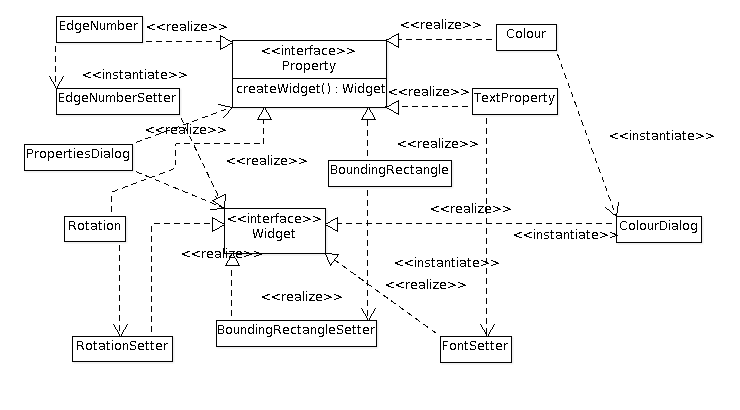
\includegraphics[scale=0.5]{images/absfactory.png}
\caption{Abstract factory}
\end{figure}
\subparagrafo{Factory:} 
\textit{Property} genera un elemento grafico per modificare una propriet\`a specifica.\\ \\
\textbf{Concrete Factory: }\\
tutte le classi che derivano da \textit{Property}. \\ \\
\textbf{Abstract Product: }\\
\textit{Widget.}\\ \\
\textbf{Concrete Product: }\\
un particolare elemento grafico a seconda della propriet\`a coinvolta. \\
\textbf{Client:}\\
\textit{PropertiesDialog.}

\newpage

\subsezione{Identificazione dei componenti architetturali di alto livello}
\subsubsezione{GUI - Intefaccia Grafica}
\begin{figure}[!ht]
\centering
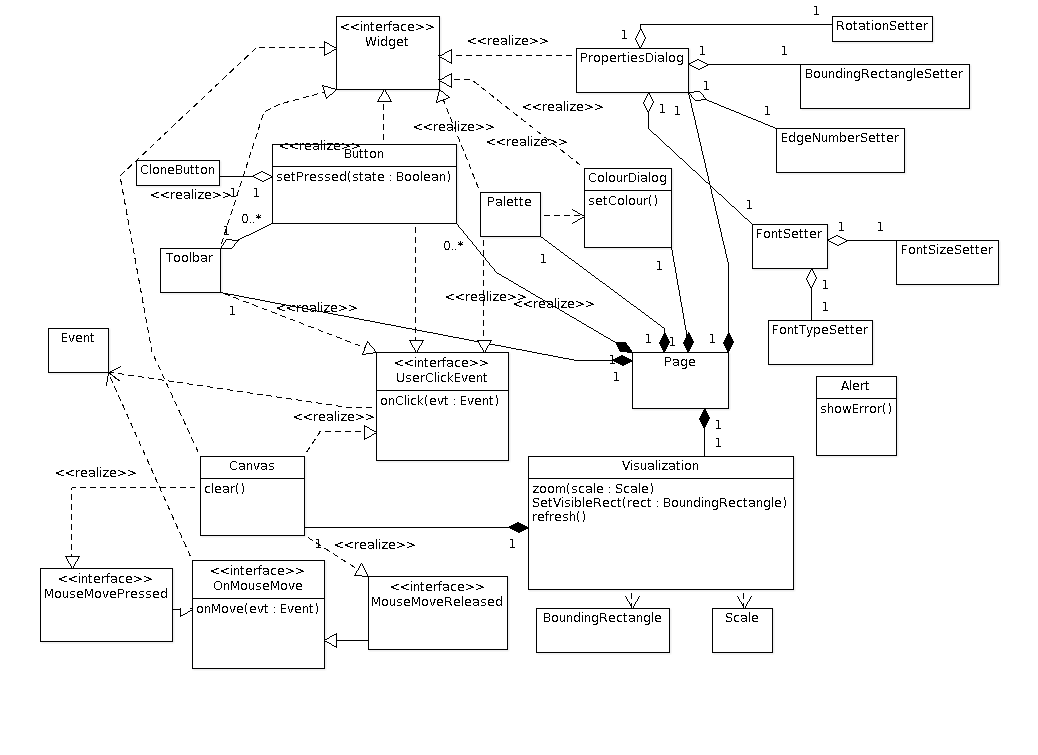
\includegraphics[scale=0.5]{images/GUIlogic.png}
\caption{GUILogic}
\end{figure}

\newpage

\begin{figure}[!ht]
\centering
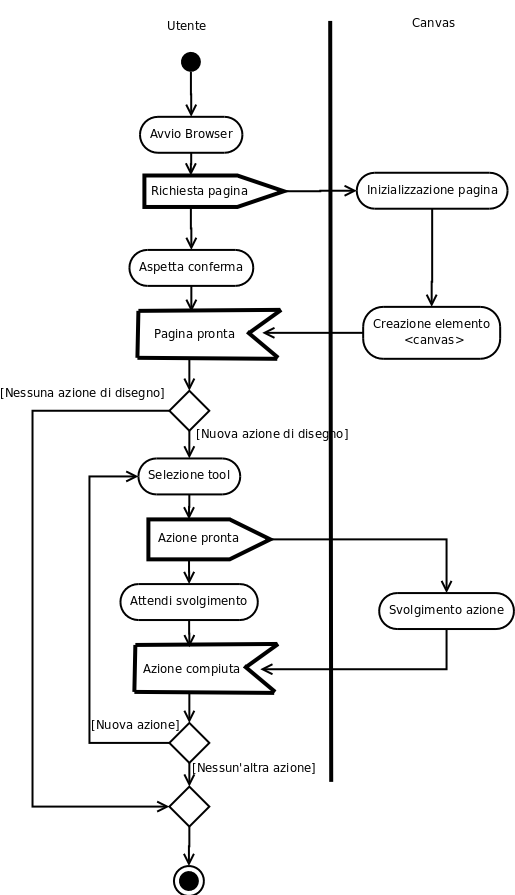
\includegraphics[scale=0.8]{images/ActivityGUI.png}
\caption{Attivit\` a: rapporto utente/canvas}
\end{figure}
\newpage

La GUI \` e  il client che verr\` a utilizzato nel sistema AJAXDRAW, e verr\` a descritta brevemente, in quanto rappresenta solo un'unit\` a che andr\`  a a lavorare sulle altre componenti di sistema. \` E costruita nella sua totalit\` a nella pagina web caricata dal browser, rappresentata dalla classe \textit{Page}, e composta da tutti i widgets con i quali interagire (che implementano tutti l'interfaccia generica \textit{Widget}).  I widgets si suddividono in \textit{Toolbar} (barra degli strumenti), \textit{Button} (pulsanti generici, che compongono anche la toolbar stessa), \textit{Palette} e \textit{ColourDialog}(per la gestione del colore), e \textit{PropertiesDialog}(per la modifica delle propriet\` a, che aggrega gli specifici \textit{Setter}). La pagina \` e composta inoltre dalla classe \textit{Visualization}, la quale gestisce il \textit{Canvas} e tutte le operazioni su di esso eseguite, tra cui la conversione tra coordinate utente e coordinate interne e lo zoom. Le classi che rappresentano oggetti con cui \`e necessario interagire tramite mouse implementano, tutte l'interfaccia \textit{UserClickEvent}, e tra queste vi \` e ovviamente la classe \textit{Canvas}, che oltre a questa implementa anche \textit{MouseMovePressed} e \textit{MouseMoveReleased}, necessarie al disegno tramite il mouse.  \` E infine presente la possibilit\` a per il programma di avvertire l'utente in caso di errore interno all'applicazione, tramite l'oggetto \textit{Alert}. \\ \\ \\

\begin{figure}[!ht]
\centering
\includegraphics[scale=0.5]{images/bozzaGUI.png}
\caption{Bozza della GUI}
\end{figure}

\newpage
\subsubsezione{ApplicationLogic - Logica interna}

\begin{figure}[!ht]
\centering
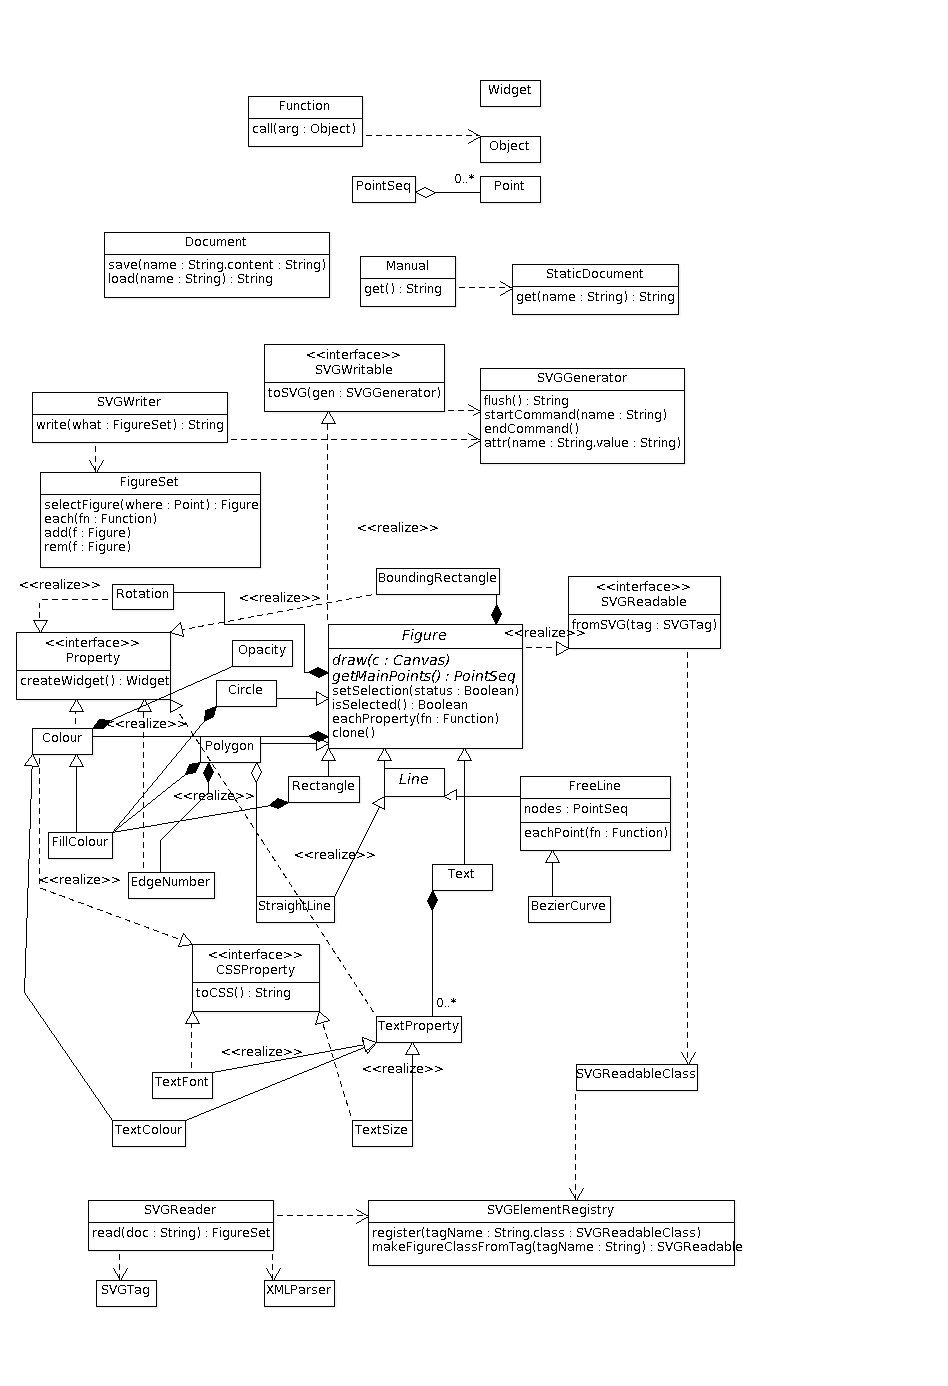
\includegraphics[scale=0.4]{images/applogic.png}
\caption{ApplicationLogic}
\end{figure}

Questo sottosistema si divide in tre ulteriori sottosistemi: la gestione delle
figure, la loro conversione in SVG e la lettura da file SVG.

\subsubsezione{Gestione figure}
\begin{figure}[!ht]
\centering
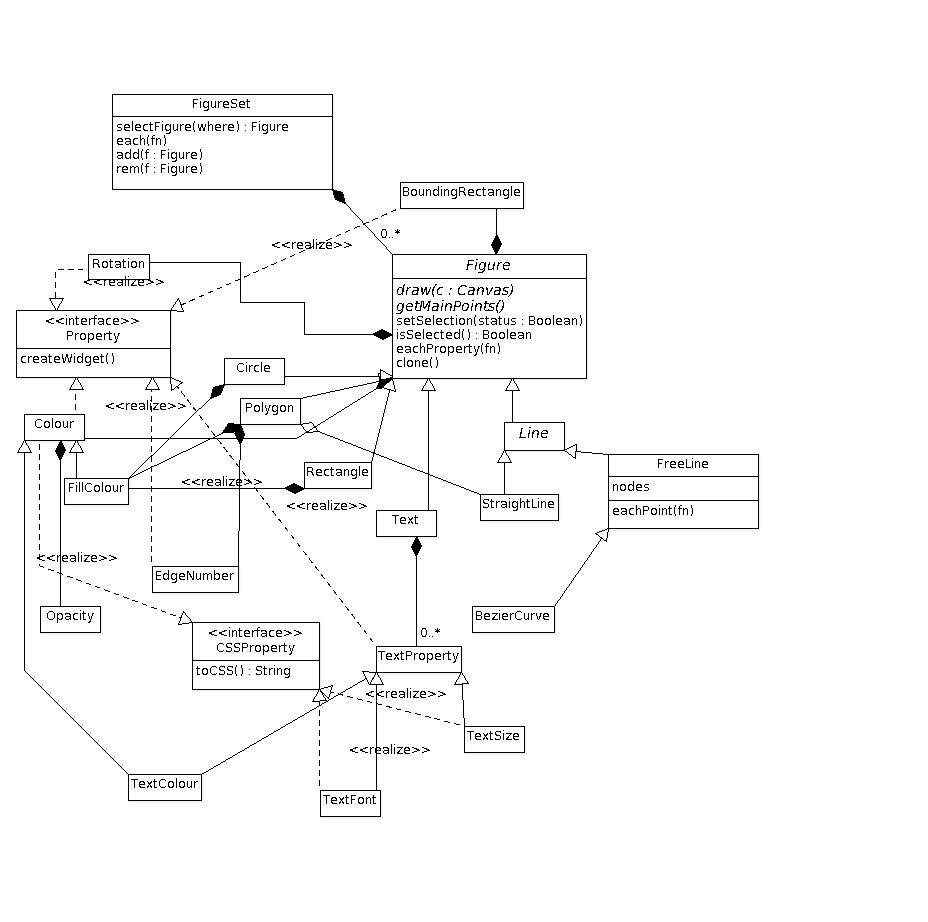
\includegraphics[scale=0.5]{images/gestionefigure.png}
\caption{Gestione figure}
\end{figure}
Si occupa della gestione interna delle figure disegnabili e manipolabili dall'utente e delle relative propriet\`a. Il termine \textit{figura} in questo contesto include anche i testi disegnati sul canvas. La classe \textit{Figure} rappresenta una figura qualsiasi. Una figura \`e caratterizzata da delle propriet\`a derivate dalla classe \textit{Property}. La suddetta classe contiene un metodo \textit{createWidget} per fabbricare un elemento grafico, il quale permette all'utente di modificare la propriet\`a che ha generato il widget stesso. Ogni figura contiene un \textit{BoundingRectangle} che rappresenta la cornice entro cui la figura \`e completamente contenuta. Una figura pu\`o essere selezionata oppure no. Le classi che implementano \textit{Figure} sono responsabili di disegnarsi sul canvas implementando il metodo \textit{draw}. In questo metodo, non si dovr\`a tener conto dell'area correntemente visualizzata o del livello di zoom, in quanto gestiti in modo trasparente dalla classe \textit{Visualization}. Ad ogni figura \`e associato un insieme di punti significativi, come ad esempio i vertici in un quadrato, ottenibili tramite il metodo \textit{getMainPoints}. Ogni figura mantiene un colore del bordo, rappresentato dalla classe \textit{Colour}. Le classi \textit{Circle}, \textit{Polygon} e \textit{Rectangle} aggiungono un ulteriore colore per il riempimento, rappresentato dalla classe \textit{FillColour}. La classe \textit{Text} rappresenta un testo disegnato dall'utente, e mantiene delle propriet\`a derivate dalla classe \textit{TextProperty}. A fini implementativi, le propriet\`a del testo e del colore andranno rappresentate secondo lo standard \textit{CSS}, quindi le suddette propriet\`a dovranno implementare l'interfaccia \textit{CSSProperty} che offre il metodo \textit{toCSS} responsabile della conversione dalla rappresentazione interna a quella \textit{CSS}. La classe \textit{FigureSet} mantiene l'insieme delle istanze di \textit{Figure} correntemente disegnate dall'utente e offre la possibilit\`a di selezionarne una a partire da un punto sul canvas.

%Parte di conversione SVG
\newpage
\subsubsezione{Conversione in \textit{SVG}}
Si occupa di trasformare il \textit{FigureSet} corrente in una stringa 
contenente un documento SVG valido e viceversa.  \\


\textbf{Da \textit{FigureSet} a SVG}

\begin{figure}[!ht]
\centering
\includegraphics[width=12cm]{images/ClassiScritturaSVG.png}
\caption{ApplicationLogic - Creazione documento SVG, diagramma delle classi}
\end{figure}

Le classi derivanti da \textit{Figure} implementano l'interfaccia \textit{SVGWritable}, che rappresenta un qualsiasi elemento convertibile in SVG. La conversione avviene tramite il metodo \textit{toSVG}. La classe \textit{SVGWriter} dovr\`a, nel metodo \textit{write}, creare un documento SVG vuoto e richiamare il metodo \textit{toSVG} su tutte le figure contenute, le quali genereranno gli elementi SVG necessari alla propria rappresentazione. Per creare un documento SVG si istanzia la classe \textit{SVGGenerator}, la quale offre dei metodi per generare comandi SVG. Quando tutte le figure hanno avuto la possibilit\`a di inserirsi nel documento SVG, il metodo \textit{flush} chiude il documento e lo ritorna sotto forma di stringa.
\newpage
\begin{figure}[!ht]
\centering
\includegraphics{images/ScritturaSVG.jpg}
\caption{ApplicationLogic - Creazione documento SVG, diagramma di sequenza}
\end{figure}

\newpage
\textbf{Da SVG a \textit{FigureSet}}

\begin{figure}[!ht]
\centering
\includegraphics[width=13cm]{images/ClassiLetturaSVG.png}
\caption{ApplicationLogic - Caricamento documento SVG, diagramma delle classi}
\end{figure}

L'importazione di un file SVG viene gestita dalla classe \textit{SVGReader} attraverso il metodo \textit{read}, che riceve un documento SVG valido sotto forma di stringa e restituisce un'istanza di \textit{FigureSet} corrispondente. Viene fatto il parsing del documento come \textit{XML} attraverso la classe \textit{XMLParser}, e per ogni comando SVG viene creato un'istanza di \textit{SVGTag} che lo rappresenta. Il nome del tag verr\`a usato come indice dal metodo \textit{makeFigureClassFromTag} della classe \textit{SVGElementRegistry}, che costruir\`a un'istanza della classe corrispondente. Su quest'istanza verr\`a invocato il metodo \textit{fromSVG}, il quale \`e responsabile di inizializzare la classe a partire dal tag. Per associare una classe al nome di un tag si usa il metodo \textit{register}. La classe registrata deve implementare l'interfaccia \textit{SVGReadable}.


\begin{figure}[!ht]
\centering
\includegraphics[width=15cm]{images/LetturaSVG.png}
\caption{ApplicationLogic - Caricamento documento SVG, diagramma di sequenza}
\end{figure}





\newpage
\subsubsezione{DocBackend - Lato Server}
\begin{figure}[!ht]
\centering
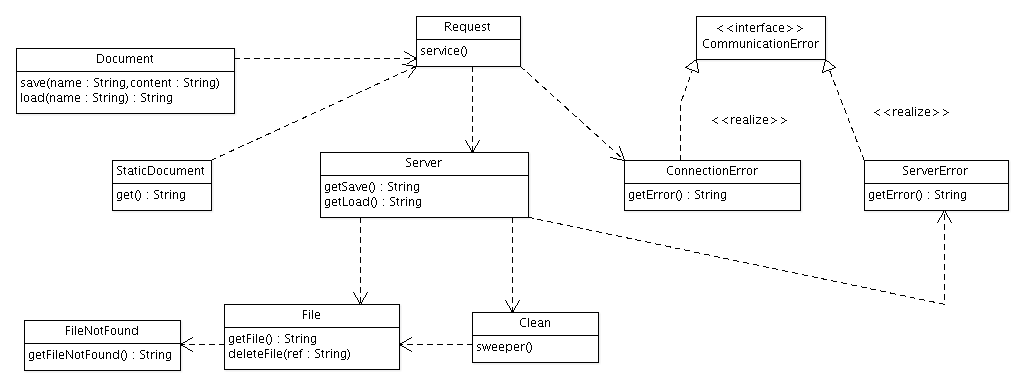
\includegraphics{images/ServerLogic.jpg}\\
\caption{ServerLogic}
\end{figure}

In AJAXDRAW \`e necessaria la presenza di una parte server, visto il modello client-server dell'applicazione. La parte server ha funzionalit\`a minimali, ma fondamentali per permettere il funzionamento dell'intero sistema. Le sue funzioni, oltre a quella di essere un webserver e fornire la pagina HTML al client, sono esclusivamente quelle di permettere un salvataggio in formato SVG del disegno effettuato sul client, effettuare il caricamento di un file risiedente su disco e avere accesso al manuale utente dell'applicazione. Come da figura 6, \`e composto da una classe \textit{Document} che rappresenta il disegno effettuato sul canvas, nella quale sono presenti i metodi \textit{save} e \textit{load}. L'uso di questi metodi permettono l'invio di una richiesta al server (classe \textit{Request}, tramite il metodo \textit{acceptRequest}). La classe \textit{Server} contiene tre metodi: \textit{getSave} che permette di salvare un file su disco, \textit{getLoad} che permette di caricare un file e \textit{getHTML} che ha il compito di ottenere la pagina HTML da fornire al client e di prelevare il manuale utente. La classe \textit{File} rappresenta un file che risiede su disco, il quale \`e possibile prelevarlo (\textit{getFile}) o cancellarlo (\textit{deleteFile}). La classe \textit{Clean} contiene il metodo \textit{sweeper} il quale elimina i file che sono gia stati scaricati o i file di client che abbandonano la connessione con il server, in modo da evitare che quesi file presenti temporaneamente sul server non lo intasino. La classe \textit{StaticDocument}, tramite il suo metodo \textit{get} permette di inviare una richiesta al server per ottenere il manuale utente. Sono presenti inoltre delle classi che permettono la gestione di eccezioni: pu\`o verificarsi un errore di comunicazione (rappresentato dall'interfaccia \textit{CommunicationError} e dalle classi \textit{ConnectionError} e \textit{ServerError} con relativi metodi che la implementano), o un errore di file non trovato (perch\`e su disco non \`e presente il file). Questo tipo di eccezione \`e rappresentato dalla classe \textit{FileNotFound} con il relativo metodo \textit{getFileError}. 


\sezione{Descrizione dei singoli componenti}
%Parte Piero
\subsezione{Widget}
\subsubsezione{Tipo, obiettivo e funzione del componente}
Rappresenta un generico oggetto grafico presente nella GUI e visibile all'utente.
\subsubsezione{Relazioni d'uso di altre componenti}
Nessuna.
\subsubsezione{Interfacce e relazioni di uso da altre componenti}
Implementata da tutti gli oggetti grafici concreti presenti nella pagina.
\subsubsezione{Attivit\`a svolte e dati trattati}
\leftskip=36pt{Nessuna a questo livello. }

\subsezione{Toolbar}
\subsubsezione{Tipo, obiettivo e funzione del componente}
Classe concreta che rappresenta la toolbar dalla quale l'utente pu\` o scegliere la funzione desiderata, posizionata in maniera da essere facilmente accessibile e sempre pronta all'uso.
\subsubsezione{Relazioni d'uso di altre componenti}
\` E formata da pi\` u istanze aggregate della classe \textit{Button}, per rappresentare ciascun tool selezionabile. Oltre a \textit{Widget}, implementa l'interfaccia \textit{UserClickEvent} per la gestione dei click del mouse. 
\subsubsezione{Interfacce e relazioni di uso da altre componenti}
\textit{Page} ne mantiene un'istanza.
\subsubsezione{Attivit\`a svolte e dati trattati}
\leftskip=36pt{Nessuna a questo livello.}

\subsezione{Button}
\subsubsezione{Tipo, obiettivo e funzione del componente}
Classe concreta che rappresenta un generico pulsante tramite il quale effettuare l'operazione desiderata.
\subsubsezione{Relazioni d'uso di altre componenti}
Oltre a \textit{Widget}, implementa l'interfaccia \textit{UserClickEvent} per la gestione dei click del mouse. 
\subsubsezione{Interfacce e relazioni di uso da altre componenti}
\textit{Page} e \textit{Toolbar }ne mantengono una o pi\` u istanze, \` e inoltre implementata dalla classe \textit{CloneButton}.
\subsubsezione{Attivit\`a svolte e dati trattati}
\begin{elencopuntato}[\normindent]
\item[-]  \textit{setPressed} metodo che valuta la pressione del bottone per decidere le operazioni da effettuare.
\end{elencopuntato}

\subsezione{CloneButton}
\subsubsezione{Tipo, obiettivo e funzione del componente}
Classe concreta che permette a un utente di clonare un oggetto presente sul canvas.
\subsubsezione{Relazioni d'uso di altre componenti}
Eredita dalla classe \textit{Button}.
\subsubsezione{Interfacce e relazioni di uso da altre componenti}
nessuna.
\subsubsezione{Attivit\`a svolte e dati trattati}
\leftskip=36pt{Nessuna a questo livello.}

\subsezione{Palette}
\subsubsezione{Tipo, obiettivo e funzione del componente}
Classe concreta che rappresenta una tavolozza composta dai colori di base pi\`u  generalmente utilizzati, nel caso l'utente non abbia bisogno di un colore specifico, la quale imposta il colore desiderato da applicare alle figure da disegnare e gi\` a disegnate semplicemente tramite la pressione della casella apposita.
\subsubsezione{Relazioni d'uso di altre componenti}
Oltre a \textit{Widget}, implementa l'interfaccia \textit{UserClickEvent} per la gestione dei click del mouse. Usa il metodo setColor della classe \textit{ColourDialog} per effettuare il cambiamento di colore alla figura.
\subsubsezione{Interfacce e relazioni di uso da altre componenti}
\textit{Page} ne mantiene un'istanza.
\subsubsezione{Attivit\`a svolte e dati trattati}
\leftskip=36pt{Nessuna a questo livello.}

\subsezione{ColourDialog}
\subsubsezione{Tipo, obiettivo e funzione del componente}
Classe concreta che rappresenta il menu di modifica dei colori di riempimento e dei bordi delle figure disegnate e da disegnare, il quale integra una ruota dei colori funzionale alla scelta di qualsiasi colore desiderato.
\subsubsezione{Relazioni d'uso di altre componenti}
Implementa \textit{Widget}.
\subsubsezione{Interfacce e relazioni di uso da altre componenti}
\textit{Page} ne mantiene un'istanza.
\subsubsezione{Attivit\`a svolte e dati trattati}
\begin{elencopuntato}[\normindent]
\item[-]  \textit{setColour} metodo che setta il colore scelto sulla figura da disegnare o selezionata sul canvas.
\end{elencopuntato}

\subsezione{PropertiesDialog}
\subsubsezione{Tipo, obiettivo e funzione del componente}
Classe concreta che rappresenta  il menu di modifica delle propriet\` a di un oggetto selezionato o da disegnare sul canvas a seconda del tipo dello stesso, che sia linea, poligono o casella di testo, ognuno con le sue caratteristiche generiche e specifiche.
\subsubsezione{Relazioni d'uso di altre componenti}
\`E formata da pi\`u istanze aggregate tra cui \textit{BoundingRectagleSetter}, \textit{EdgeNumberSetter} e \textit{FontSetter}. Implementa \textit{Widget}.
\subsubsezione{Interfacce e relazioni di uso da altre componenti}
\textit{Page} ne mantiene un'istanza.
\subsubsezione{Attivit\`a svolte e dati trattati}
\leftskip=36pt{Nessuna a questo livello.}

\subsezione{BoundingRectagleSetter}
\subsubsezione{Tipo, obiettivo e funzione del componente}
Classe concreta che rappresenta l'oggetto che si occupa di impostare e modificare le coordinate del rettangolo contenente la figura disegnata sul canvas.
\subsubsezione{Relazioni d'uso di altre componenti}
Nessuna.
\subsubsezione{Interfacce e relazioni di uso da altre componenti}
\textit{PropertiesDialog} ne mantiene un'istanza.
\subsubsezione{Attivit\`a svolte e dati trattati}
\leftskip=36pt{Nessuna a questo livello.}

\subsezione{EdgeNumberSetter}
\subsubsezione{Tipo, obiettivo e funzione del componente}
Classe concreta che rappresenta l'oggetto che si occupa di modificare il numero di lati della figura da disegnare o selezionata.
\subsubsezione{Relazioni d'uso di altre componenti}
Nessuna.
\subsubsezione{Interfacce e relazioni di uso da altre componenti}
\textit{PropertiesDialog} ne mantiene un'istanza.
\subsubsezione{Attivit\`a svolte e dati trattati}
\leftskip=36pt{Nessuna a questo livello.}

\subsezione{RotationSetter}
\subsubsezione{Tipo, obiettivo e funzione del componente}
Classe concreta che permette a un utente di ruotare un oggetto presente sul canvas
\subsubsezione{Relazioni d'uso di altre componenti}
nessuna. 
\subsubsezione{Interfacce e relazioni di uso da altre componenti}
\textit{PropertiesDialog} ne mantiene un' istanza.
\subsubsezione{Attivit\`a svolte e dati trattati}
\leftskip=36pt{Nessuna a questo livello.}

\subsezione{FontSetter}
\subsubsezione{Tipo, obiettivo e funzione del componente}
Classe concreta che rappresenta l'oggetto che si occupa di modificare il font di una casella di testo da disegnare o selezionata.
\subsubsezione{Relazioni d'uso di altre componenti}
\` E formata dalle istanze aggregate di \textit{FontSizeSetter} e \textit{FontTypeSetter}.
\subsubsezione{Interfacce e relazioni di uso da altre componenti}
\textit{PropertiesDialog} ne mantiene un'istanza.
\subsubsezione{Attivit\`a svolte e dati trattati}
\leftskip=36pt{Nessuna a questo livello.}

\subsezione{FontSizeSetter}
\subsubsezione{Tipo, obiettivo e funzione del componente}
Classe concreta che rappresenta l'oggetto che si occupa di modificare la dimensione del carattere di una casella di testo da disegnare o selezionata.
\subsubsezione{Relazioni d'uso di altre componenti}
Nessuna.
\subsubsezione{Interfacce e relazioni di uso da altre componenti}
\textit{FontSetter} ne mantiene un'istanza.
\subsubsezione{Attivit\`a svolte e dati trattati}
\leftskip=36pt{Nessuna a questo livello.}

\subsezione{FontTypeSetter}
\subsubsezione{Tipo, obiettivo e funzione del componente}
Classe concreta che rappresenta l'oggetto che si occupa di modificare il tipo di carattere di una casella di testo da disegnare o selezionata, scegliendo tra alcune famiglie predefinite.
\subsubsezione{Relazioni d'uso di altre componenti}
Nessuna.
\subsubsezione{Interfacce e relazioni di uso da altre componenti}
\textit{FontSetter} ne mantiene un'istanza.
\subsubsezione{Attivit\`a svolte e dati trattati}
\leftskip=36pt{Nessuna a questo livello.}

\subsezione{UserClickEvent}
\subsubsezione{Tipo, obiettivo e funzione del componente}
Rappresenta la risposta ad un click dell'utente su un oggetto che implementa tale intefaccia.
\subsubsezione{Relazioni d'uso di altre componenti}
Utilizza un generico evento, istanza della classe \textit{Event}, per la gestione del click del mouse.
\subsubsezione{Interfacce e relazioni di uso da altre componenti}
\`E implementata dalle classi \textit{Toolbar}, \textit{Palette}, \textit{Canvas}, e \textit{Button}. 
\subsubsezione{Attivit\`a svolte e dati trattati}
\begin{elencopuntato}[\normindent]
\item[-]  \textit{onClick} gestisce la pressione del pulsante del mouse su un oggetto che implementa l'interfaccia.
\end{elencopuntato}

\subsezione{Canvas}
\subsubsezione{Tipo, obiettivo e funzione del componente}
Classe che rappresenta il canvas, oggetto sul quale verrano visualizzate le figure disegnate, modificate e spostate dall'utente, tramite l'utilizzo del mouse. 
\subsubsezione{Relazioni d'uso di altre componenti}
Implementa le interfacce \textit{MouseMovePressed} e \textit{MouseMoveReleased}, per tenere traccia della pressione del pulsante sinistro del mouse e del suo trascinamento, oltre a \textit{Widget}.
\subsubsezione{Interfacce e relazioni di uso da altre componenti}
Compone un'istanza di \textit{Visualization}, che si occupa della sua visualizzazione su schermo.
\subsubsezione{Attivit\`a svolte e dati trattati}
\begin{elencopuntato}[\normindent]
\item[-]  \textit{clear} imposta il canvas alla sua condizione iniziale.
\end{elencopuntato}

\subsezione{OnMouseMove}
\subsubsezione{Tipo, obiettivo e funzione del componente}
Rappresenta un generico stato di utilizzo del mouse, specificato meglio dalle interfacce che la estendono.
\subsubsezione{Relazioni d'uso di altre componenti}
Utilizza un'istanza della classe \textit{Event}.
\subsubsezione{Interfacce e relazioni di uso da altre componenti}
\` E esteso dalle interfacce \textit{MouseMovePressed} e \textit{MouseMoveReleased}, per la gestione pi\` u specifica della pressione del pulsante sinistro del mouse.
\subsubsezione{Attivit\`a svolte e dati trattati}
\begin{elencopuntato}[\normindent]
\item[-]  \textit{onMove} gestisce il generico movimento del mouse.
\end{elencopuntato}

\subsezione{MouseMovePressed}
\subsubsezione{Tipo, obiettivo e funzione del componente}
Rappresenta lo stato di pressione del pulsante sinistro del mouse, utile in genere per il dimensionamento di una figura in fase di creazione, del suo ridimensionamento o del suo spostamento sul canvas. 
\subsubsezione{Relazioni d'uso di altre componenti}
Estende \textit{OnMouseMove}.
\subsubsezione{Interfacce e relazioni di uso da altre componenti}
Viene implementato dall'istanza della classe \textit{Canvas}, per gestire il caso del pulsante del mouse premuto.
\subsubsezione{Attivit\`a svolte e dati trattati}
\leftskip=36pt{Nessuna a questo livello.}

\subsezione{MouseMoveReleased}
\subsubsezione{Tipo, obiettivo e funzione del componente}
Rappresenta lo stato di rilascio del pulsante sinistro del mouse a seguito della sua pressione, che in genere sta ad indicare il termine di un'azione effettuata sul canvas.
\subsubsezione{Relazioni d'uso di altre componenti}
Estende \textit{OnMouseMovePressed}.
\subsubsezione{Interfacce e relazioni di uso da altre componenti}
Viene implementato dall'istanza della classe \textit{Canvas}, per gestire il caso del pulsante del mouse premuto.
\subsubsezione{Attivit\`a svolte e dati trattati}
\leftskip=36pt{Nessuna a questo livello.}

\subsezione{Event}
\subsubsezione{Tipo, obiettivo e funzione del componente}
Classe che rappresenta un generico evento generato da un'azione prestabilita, quali movimenti e pressione dei tasti del mouse.
\subsubsezione{Relazioni d'uso di altre componenti}
Nessuna.
\subsubsezione{Interfacce e relazioni di uso da altre componenti}
Viene utilizzato dalle interfacce \textit{OnMouseMove} e \textit{UserClickEvent}, a seguito dell'utilizzo del mouse per effettuare qualche operazione.
\subsubsezione{Attivit\`a svolte e dati trattati}
\leftskip=36pt{Nessuna a questo livello.}

\subsezione{Page}
\subsubsezione{Tipo, obiettivo e funzione del componente}
Classe concreta che rappresenta la pagina web visualizzata dall'utente tramite l'internet browser, contenitore di tutti i widgets componenti l'interfaccia.
\subsubsezione{Relazioni d'uso di altre componenti}
\` E composta da istanze delle classi \textit{Toolbar}, \textit{Button}, \textit{Palette}, \textit{ColourDialog}, \textit{PropertiesDialog} e \textit{Visualization}.
\subsubsezione{Interfacce e relazioni di uso da altre componenti}
Nessuna.
\subsubsezione{Attivit\`a svolte e dati trattati}
\leftskip=36pt{Nessuna a questo livello.}

\subsezione{Visualization}
\subsubsezione{Tipo, obiettivo e funzione del componente}
Classe concreta che si occupa delle operazioni di visualizzazione del canvas su schermo, come la riscalatura a seguito di uno zoom e la corretta visualizzazione della parte ingrandita o rimpicciolita.
\subsubsezione{Relazioni d'uso di altre componenti}
\` E composta da un'istanza della classe \textit{Canvas}. Utilizza istanze di \textit{Scale} e \textit{BoundingRectangle}.
\subsubsezione{Interfacce e relazioni di uso da altre componenti}
\textit{Page} ne mantiene un'istanza.
\subsubsezione{Attivit\`a svolte e dati trattati}
\begin{elencopuntato}[\normindent]
\item[-]  \textit{zoom} metodo che si occupa del riscalamento a seguito di uno zoom sul canvas.
\item[-]  \textit{setVisibleRect} metodo usato per settare l'area di canvas visualizzata.
\item[-]  \textit{refresh} si occupa dell'aggiornamento della situazione del canvas visualizzato.
\end{elencopuntato}

\subsezione{Scale}
\subsubsezione{Tipo, obiettivo e funzione del componente}
Classe concreta che si occupa delle operazioni di riscalamento del canvas su schermo. 
\subsubsezione{Relazioni d'uso di altre componenti}
Nessuna.
\subsubsezione{Interfacce e relazioni di uso da altre componenti}
\textit{Visualization} ne utilizza un'istanza.
\subsubsezione{Attivit\`a svolte e dati trattati}
\leftskip=36pt{Nessuna a questo livello.}

\subsezione{Alert}
\subsubsezione{Tipo, obiettivo e funzione del componente}
Classe concreta che si occupa di avvertire l'utente di un errore verificatosi nel programma.
\subsubsezione{Relazioni d'uso di altre componenti}
Nessuna.
\subsubsezione{Interfacce e relazioni di uso da altre componenti}
Nessuna.
\subsubsezione{Attivit\`a svolte e dati trattati}
\begin{elencopuntato}[\normindent]
\item[-]  \textit{showError} metodo che avverte l'utente di un qualche errore tramite pop-up o un avviso di altro genere.
\end{elencopuntato}


%Parte Dissegna
\subsezione{Figure}
\subsubsezione{Tipo, obiettivo e funzione del componente}
Classe astratta che rappresenta una figura generica nel sistema, ovvero un oggetto disegnabile nel canvas.
\subsubsezione{Relazioni d'uso di altre componenti}
Mantiene un'istanza della classe \textit{BoundingRectangle} per rappresentare i limiti della figura. Contiene anche un'istanza di \textit{Colour} che rappresenta il colore del bordo. Deriva, ma non implementa, l'interfaccia \textit{SVGReadable} e l'interfaccia \textit{SVGWritable}, in quanto le sue sottoclassi dovranno essere serializzabili e deserializabili in file SVG.
\subsubsezione{Interfacce e relazioni di uso da altre componenti}
Viene aggregata dalla classe \textit{FigureSet}.
\subsubsezione{Attivit\`a svolte e dati trattati}
\begin{elencopuntato}[\normindent]
\item[-]  \textit{draw} metodo astratto per disegnare la figura sul canvas.
\item[-]  \textit{getMainPoints} metodo astratto per ottenere i punti della figura manipolabili dall'utente.
\item[-]  \textit{setSelection} permette di selezionare/deselezionare la figura.
\item[-]  \textit{isSelected} dice se la figura \`e correntemente selezionata.
\item[-]  \textit{eachProperty} applica la funzione fn ad ogni propriet\`a della figura.
\item[-]  \textit{clone} crea un oggetto clone appena sopra la figura.
\end{elencopuntato}

\subsezione{FigureSet}
\subsubsezione{Tipo, obiettivo e funzione del componente}
Rappresenta una collezione di figure. Tutte le figure disegnate dall'utente sono contenute in questa collezione, la quale ne permette la manipolazione e l'attraversamento. Per cancellare una figura \`e sufficiente rimuoverla dalla collezione.
\subsubsezione{Relazioni d'uso di altre componenti}
Contiene le istanze di \textit{Figure} correntemente attive.
\subsubsezione{Interfacce e relazioni di uso da altre componenti}
Usata dalla classe \textit{SVGWriter} per serializzare in SVG le figure correnti a dall'interfaccia utente per accedere alle figure. Pu\`o venire generata dalla classe \textit{SVGReader} dopo la deserializzazione di un file SVG.
\subsubsezione{Attivit\`a svolte e dati trattati}
\begin{elencopuntato}[\normindent]
\item[-]  \textit{selectFigure} permette di selezionare una figura contenente il punto passato come argomento, se tale figura esiste.
\item[-]  \textit{each} permette di applicare una funzione ad ogni figura. Viene usato per iterare attraverso la collezione.
\item[-]  \textit{add} aggiunge una figura all'insieme.
\item[-]  \textit{rem} rimuove una figura dall'insieme, se presente.
\end{elencopuntato}

\subsezione{Property}
\subsubsezione{Tipo, obiettivo e funzione del componente}
Rappresenta una propriet\`a generica di una figura. Le propriet\`a influenzano 
l'aspetto delle diverse figure, e sono modificabili dall'utente.
\subsubsezione{Relazioni d'uso di altre componenti}
Nessuna.
\subsubsezione{Interfacce e relazioni di uso da altre componenti}
Implementata da tutte le propriet\`a concrete delle diverse figure.
\subsubsezione{Attivit\`a svolte e dati trattati}
\begin{elencopuntato}[\normindent]
\item[-] \textit{createWidget} crea un widget grafico che permetter\`a all'utente di modificare la propriet\`a.
\end{elencopuntato}

\subsezione{CSSProperty}
\subsubsezione{Tipo, obiettivo e funzione del componente}
Rappresenta una propriet\`a di una figura che necessita di una rappresentazione conforme ai CSS. Questa rappresentazione \`e necessaria per applicare alcune propriet\`a (come ad esempio il colore) al canvas e per la conversione in SVG.
\subsubsezione{Relazioni d'uso di altre componenti}
Nessuna.
\subsubsezione{Interfacce e relazioni di uso da altre componenti}
Implementata da \textit{Colour}, \textit{TextFont} e \textit{TextSize}. 
\subsubsezione{Attivit\`a svolte e dati trattati}
\begin{elencopuntato}[\normindent]
\item[-] \textit{toCSS} genera una stringa che rappresenta la propriet\`a come propriet\`a CSS.
\end{elencopuntato}

\subsezione{Opacity}
\subsubsezione{Tipo, obiettivo e funzione del componente}
Rappresenta l'opacit\`a di un colore. Mantiene un unico valore che varia nell'intervallo [0, 1]. Se il valore \`e 0 la figura \`e completamente trasparente, se
il valore \`e 1, la figura \`e completamente opaca, ovvero non permette la visualizzazione delle figure sottostanti.
\subsubsezione{Relazioni d'uso di altre componenti}
Nessuna.
\subsubsezione{Interfacce e relazioni di uso da altre componenti}
\textit{Colour} ne mantiene un'istanza.
\subsubsezione{Attivit\`a svolte e dati trattati}
\leftskip=36pt{Nessuna a questo livello.}

\subsezione{EdgeNumber}
\subsubsezione{Tipo, obiettivo e funzione del componente}
Rappresenta il numero degli spigoli di un poligono. Questo numero non pu\`o essere inferiore a 3.
\subsubsezione{Relazioni d'uso di altre componenti}
Implementa \textit{Property}.
\subsubsezione{Interfacce e relazioni di uso da altre componenti}
\textit{Polygon} ne mantiene un'istanza.
\subsubsezione{Attivit\`a svolte e dati trattati}
\leftskip=36pt{Nessuna a questo livello.}

\subsezione{Colour}
\subsubsezione{Tipo, obiettivo e funzione del componente}
Rappresenta un colore come una terna RGB pi\`u l'opacit\`a del colore stesso. Questa rappresentazione trova una corrispondenza diretta sia nel tag <canvas>, sia nel formato SVG.
\subsubsezione{Relazioni d'uso di altre componenti}
Implementa \textit{Property} e \textit{CSSProperty}. Mantiene un'istanza di \textit{Opacity} che rappresenta l'opacit\`a del colore.
\subsubsezione{Interfacce e relazioni di uso da altre componenti}
\textit{Figure} ne mantiene un'istanza per rappresentare il colore del bordo.
\subsubsezione{Attivit\`a svolte e dati trattati}
\leftskip=36pt{Nessuna a questo livello.}

\subsezione{FillColour}
\subsubsezione{Tipo, obiettivo e funzione del componente}
Rappresenta un colore di riempimento.
\subsubsezione{Relazioni d'uso di altre componenti}
Deriva da \textit{Colour}.
\subsubsezione{Interfacce e relazioni di uso da altre componenti}
\textit{Circle}, \textit{Polygon} e \textit{Rectangle} ne mantengono un'istanza.
\subsubsezione{Attivit\`a svolte e dati trattati}
\leftskip=36pt{Nessuna a questo livello.}

\subsezione{TextProperty}
\subsubsezione{Tipo, obiettivo e funzione del componente}
Propriet\`a di un testo grafico.
\subsubsezione{Relazioni d'uso di altre componenti}
Deriva da \textit{Property}.
\subsubsezione{Interfacce e relazioni di uso da altre componenti}
\textit{Text} ne mantiene delle istanze.
\subsubsezione{Attivit\`a svolte e dati trattati}
\leftskip=36pt{Nessuna a questo livello.}

\subsezione{TextColour}
\subsubsezione{Tipo, obiettivo e funzione del componente}
Rappresenta il colore di un testo.
\subsubsezione{Relazioni d'uso di altre componenti}
Deriva da \textit{Colour} e da \textit{TextProperty}.
\subsubsezione{Interfacce e relazioni di uso da altre componenti}
Nessuna.
\subsubsezione{Attivit\`a svolte e dati trattati}
\leftskip=36pt{Nessuna a questo livello.}

\subsezione{TextFont}
\subsubsezione{Tipo, obiettivo e funzione del componente}
Rappresenta il font di un testo. Mantiene il nome del font.
\subsubsezione{Relazioni d'uso di altre componenti}
Deriva da \textit{TextProperty} e implementa \textit{CSSProperty}.
\subsubsezione{Interfacce e relazioni di uso da altre componenti}
Nessuna.
\subsubsezione{Attivit\`a svolte e dati trattati}
\leftskip=36pt{Nessuna a questo livello.}

\subsezione{TextSize}
\subsubsezione{Tipo, obiettivo e funzione del componente}
Rappresenta la grandezza di un testo. La grandezza viene espressa in pixel.
\subsubsezione{Relazioni d'uso di altre componenti}
Deriva da \textit{TextProperty} e implementa \textit{CSSProperty}.
\subsubsezione{Interfacce e relazioni di uso da altre componenti}
Nessuna.
\subsubsezione{Attivit\`a svolte e dati trattati}
\leftskip=36pt{Nessuna a questo livello.}

\subsezione{BoundingRectangle}
\subsubsezione{Tipo, obiettivo e funzione del componente}
Rappresenta la posizione e le dimensioni massime di una figura. Modificando il
\textit{BoundingRectangle} \`e possibile spostare, ingrandire e deformare una figura.
\`E responsabilit\`a delle singole figure, all'interno del metodo \textit{draw}, di disegnarsi all'interno dei limiti.
\subsubsezione{Relazioni d'uso di altre componenti}
Implementa \textit{Property}. Ogni istanza di \textit{Figure} ne mantiene un'istanza.
\subsubsezione{Interfacce e relazioni di uso da altre componenti}
Nessuna.
\subsubsezione{Attivit\`a svolte e dati trattati}
\leftskip=36pt{Nessuna a questo livello.}

\subsezione{Rotation}
\subsubsezione{Tipo, obiettivo e funzione del componente}
Propriet\`a che rappresenta il grado di rotazione di una figura. La rotazione avviene seguendo il centro della circonferenza che iscrive la figura; pi\`u precisamente, la rotazione viene svolta attraverso l'uso del centro del BoundingRectangle. 
\subsubsezione{Relazioni d'uso di altre componenti}
Deriva da \textit{Property}.
\subsubsezione{Interfacce e relazioni di uso da altre componenti}
\textit{figure} ne mantiene una o pi\'u istanze.
\subsubsezione{Attivit\`a svolte e dati trattati}
\leftskip=36pt{Nessuna a questo livello.}

\subsezione{Circle}
\subsubsezione{Tipo, obiettivo e funzione del componente}
Rappresenta un cerchio o un'ellisse, a seconda che il proprio \textit{BoundingRectangle} sia un quadrato oppure un rettangolo. Viene disegnato in modo da essere inscritto al \textit{BoundingRectangle}.
\subsubsezione{Relazioni d'uso di altre componenti}
Deriva da \textit{Figure} e ne implementa i metodi astratti. Mantiene un'istanza di \textit{FillColour}.
\subsubsezione{Interfacce e relazioni di uso da altre componenti}
Nessuna.
\subsubsezione{Attivit\`a svolte e dati trattati}
\leftskip=36pt{Nessuna a questo livello.}

\subsezione{Rectangle}
\subsubsezione{Tipo, obiettivo e funzione del componente}
Rappresenta un rettangolo od un quadrato.
\subsubsezione{Relazioni d'uso di altre componenti}
Deriva da \textit{Figure} e ne implementa i metodi astratti. Mantiene un'istanza di \textit{FillColour}.
\subsubsezione{Interfacce e relazioni di uso da altre componenti}
Nessuna.
\subsubsezione{Attivit\`a svolte e dati trattati}
\leftskip=36pt{Nessuna a questo livello.}

\subsezione{Line}
\subsubsezione{Tipo, obiettivo e funzione del componente}
Rappresenta una linea generica.
\subsubsezione{Relazioni d'uso di altre componenti}
Deriva da \textit{Figure}.
\subsubsezione{Interfacce e relazioni di uso da altre componenti}
Nessuna.
\subsubsezione{Attivit\`a svolte e dati trattati}
\leftskip=36pt{Nessuna a questo livello.}

\subsezione{StraightLine}
\subsubsezione{Tipo, obiettivo e funzione del componente}
Rappresenta una linea diritta. La linea v\`a dall'angolo in alto a sinistra all'angolo in basso a destra del \textit{BoundingRectangle}.
\subsubsezione{Relazioni d'uso di altre componenti}
Deriva da \textit{Line} e ne implementa i metodi astratti.
\subsubsezione{Interfacce e relazioni di uso da altre componenti}
Nessuna.
\subsubsezione{Attivit\`a svolte e dati trattati}
\leftskip=36pt{Nessuna a questo livello.}

\subsezione{FreeLine}
\subsubsezione{Tipo, obiettivo e funzione del componente}
Rappresenta una linea a mano libera. Viene implementata tramite delle curve di bezier brevi e ravvicinate tra di loro.
\subsubsezione{Relazioni d'uso di altre componenti}
Deriva da \textit{Line} e ne implementa i metodi astratti. Mantiene una lista di punti. I punti prendono come origine l'angolo in alto a sinistra del \textit{BoundingRectangle} e presuppongono un quadrato alto 1 e largo 1, in modo da essere indipendenti dal \textit{BoundingRectangle}. I punti verranno poi convertiti nei loro valori assoluti, a seconda del \textit{BoundingRectangle}, prima di disegnare la linea. Qualora ripetere questa computazione ad ogni refresh fosse troppo dispendioso, si potrebbe ricorrere ad un sistema di caching.
\subsubsezione{Interfacce e relazioni di uso da altre componenti}
Usata come base da \textit{BezierCurve}.
\subsubsezione{Attivit\`a svolte e dati trattati}
\begin{elencopuntato}[\normindent]
\item[-] \textit{eachPoint} applica una funzione ad ogni nodo della linea.
\end{elencopuntato}

\subsezione{BezierCurve}
\subsubsezione{Tipo, obiettivo e funzione del componente}
Rappresenta una linea curva, disegnata tramite curve di bezier.
\subsubsezione{Relazioni d'uso di altre componenti}
Deriva da \textit{FreeLine}. A differenza di \textit{FreeLine} la lista di punti interni contiene un numero ridotto di punti.
\subsubsezione{Interfacce e relazioni di uso da altre componenti}
Nessuna.
\subsubsezione{Attivit\`a svolte e dati trattati}
\leftskip=36pt{Nessuna a questo livello.}

\subsezione{Polygon}
\subsubsezione{Tipo, obiettivo e funzione del componente}
Rappresenta un poligono regolare.
\subsubsezione{Relazioni d'uso di altre componenti}
Deriva da \textit{Figure} e ne implementa i metodi astratti. Mantiene un'istanza di \textit{FillColour} e di \textit{EdgeNumber} che ne identifica il numero di lati.
\subsubsezione{Interfacce e relazioni di uso da altre componenti}
Nessuna.
\subsubsezione{Attivit\`a svolte e dati trattati}
\leftskip=36pt{Nessuna a questo livello.}

\subsezione{SVGWriter}
\subsubsezione{Tipo, obiettivo e funzione del componente}
Permette di creare un documento SVG.
\subsubsezione{Relazioni d'uso di altre componenti}
Accede alle figure correnti attraverso un'istanza di \textit{FigureSet}.
\subsubsezione{Interfacce e relazioni di uso da altre componenti}
Nessuna.
\subsubsezione{Attivit\`a svolte e dati trattati}
\begin{elencopuntato}[\normindent]
\item[-] \textit{write} crea un documento SVG che contiene le figure correntemente disegnate.
\end{elencopuntato}

\subsezione{SVGWritable}
\subsubsezione{Tipo, obiettivo e funzione del componente}
Rappresenta un oggetto convertibile in SVG.
\subsubsezione{Relazioni d'uso di altre componenti}
Usa \textit{SVGGenerator} per generare i comandi SVG.
\subsubsezione{Interfacce e relazioni di uso da altre componenti}
Implementata dalle classi che rappresentano figure.
\subsubsezione{Attivit\`a svolte e dati trattati}
\begin{elencopuntato}[\normindent]
\item[-] \textit{toSVG} converte in SVG. Per trascriversi in un documento SVG l'oggetto potr\`a usare solo i metodi messi a disposizione dall'\textit{SVGGenerator} passato come parametro.
\end{elencopuntato}

\subsezione{SVGGenerator}
\subsubsezione{Tipo, obiettivo e funzione del componente}
Rappresenta un documento SVG in costruzione. Mantiene al suo interno una rappresentazione del documento finora generato e mette a disposizione dei metodi per scrivere nel documento.
\subsubsezione{Relazioni d'uso di altre componenti}
Nessuna.
\subsubsezione{Interfacce e relazioni di uso da altre componenti}
Usato da \textit{SVGWriter} e dalle classi che implementano \textit{SVGWritable} per realizzare un documento SVG.
\subsubsezione{Attivit\`a svolte e dati trattati}
\begin{elencopuntato}[\normindent]
\item[-] \textit{startCommand} apre un comando con il nome dato.
\item[-] \textit{attr} aggiunge un attributo con il nome e il valore dato al comando corrente.
\item[-] \textit{endCommand} chiude il comando corrente.
\item[-] \textit{flush} ritorna il documento finora generato sotto forma di stringa.
\end{elencopuntato}

\subsezione{XMLParser}
\subsubsezione{Tipo, obiettivo e funzione del componente}
Un parser SVG. Costruisce il DOM di un documento XML a partire dalla sua rappresentazione testuale.
\subsubsezione{Relazioni d'uso di altre componenti}
Nessuna.
\subsubsezione{Interfacce e relazioni di uso da altre componenti}
Usato da \textit{SVGReader}.
\subsubsezione{Attivit\`a svolte e dati trattati}
\leftskip=36pt{Nessuna a questo livello.}

\subsezione{SVGTag}
\subsubsezione{Tipo, obiettivo e funzione del componente}
Rappresenta un tag (ovvero un comando) SVG. Un tag \`e caratterizzato dal nome, da un'insieme di coppie attributo-valore, e da eventuali tag figli.
\subsubsezione{Relazioni d'uso di altre componenti}
Nessuna.
\subsubsezione{Interfacce e relazioni di uso da altre componenti}
Usato da \textit{SVGReader} e dalle classi che implementano \textit{SVGReadable}.
\subsubsezione{Attivit\`a svolte e dati trattati}
\leftskip=36pt{Nessuna a questo livello.}

\subsezione{SVGReadable}
\subsubsezione{Tipo, obiettivo e funzione del componente}
Rappresenta un oggetto caricabile da un documento SVG.
\subsubsezione{Relazioni d'uso di altre componenti}
Nessuna.
\subsubsezione{Interfacce e relazioni di uso da altre componenti}
Implementata dalle classi che rappresentano figure.
\subsubsezione{Attivit\`a svolte e dati trattati}
\begin{elencopuntato}[\normindent]
\item[-] \textit{fromSVG} inizializza, modificando il proprio stato interno, se stesso a partire da un tag SVG.
\end{elencopuntato}

\subsezione{SVGReadableClass}
\subsubsezione{Tipo, obiettivo e funzione del componente}
Metaclasse di \textit{SVGReadable}.
\subsubsezione{Relazioni d'uso di altre componenti}
Nessuna.
\subsubsezione{Interfacce e relazioni di uso da altre componenti}
Usata da \textit{SVGElementRegistry} per associare il nome di un tag a una classe che implementa \textit{SVGReadable}.
\subsubsezione{Attivit\`a svolte e dati trattati}
\leftskip=36pt{Nessuna a questo livello.}

\subsezione{SVGReader}
\subsubsezione{Tipo, obiettivo e funzione del componente}
Permette di caricare un documento SVG.
\subsubsezione{Relazioni d'uso di altre componenti}
Usa \textit{XMLParser} per fare il parsing del documento testuale, crea \textit{SVGTag} e usa \textit{SVGElementRegistry} per creare una figura a partire da un tag SVG.
\subsubsezione{Interfacce e relazioni di uso da altre componenti}
Nessuna.
\subsubsezione{Attivit\`a svolte e dati trattati}
\begin{elencopuntato}[\normindent]
\item[-] \textit{read} prende un documento SVG e ritorna un'istanza di \textit{FigureSet} che lo rappresenta.
\end{elencopuntato}

\subsezione{SVGElementRegistry}
\subsubsezione{Tipo, obiettivo e funzione del componente}
Associa nomi di tag SVG a classi (non istanze) che implementano \textit{SVGReadable} e ne permette l'istanziazione. 
\subsubsezione{Relazioni d'uso di altre componenti}
Usa \textit{SVGReadableClass} per mantenere un riferimento ad una classe per poterla poi istanziare.
\subsubsezione{Interfacce e relazioni di uso da altre componenti}
Usata da \textit{SVGReader} durante la conversione di un documento SVG per creare oggetti del tipo corretto a partire da un tag SVG. Gli oggetti creati andranno poi inizializzati. Ogni classe che implementa \textit{SVGReadable} deve registrarsi.
\subsubsezione{Attivit\`a svolte e dati trattati}
\begin{elencopuntato}[\normindent]
\item[-] \textit{register} associa il nome di un tag SVG ad una classe che implementa \textit{SVGReadable}.
\item[-] \textit{makeFigureClassFromTag} crea un'istanza della classe associata al nome di tag passato come parametro.
\end{elencopuntato}

\subsezione{Manual}
\subsubsezione{Tipo, obiettivo e funzione del componente}
Rappresenta il manuale utente.
\subsubsezione{Relazioni d'uso di altre componenti}
Usa \textit{StaticDocument} per ottenere il file contenente il manuale.
\subsubsezione{Interfacce e relazioni di uso da altre componenti}
Nessuna.
\subsubsezione{Attivit\`a svolte e dati trattati}
\begin{elencopuntato}[\normindent]
\item[-] \textit{get} ritorna il manuale.
\end{elencopuntato}

\subsezione{Point}
\subsubsezione{Tipo, obiettivo e funzione del componente}
Un punto sul piano.
\subsubsezione{Relazioni d'uso di altre componenti}
Nessuna.
\subsubsezione{Interfacce e relazioni di uso da altre componenti}
Nessuna.
\subsubsezione{Attivit\`a svolte e dati trattati}
\leftskip=36pt{Nessuna a questo livello.}

\subsezione{PointSeq}
\subsubsezione{Tipo, obiettivo e funzione del componente}
Una sequenza di \textit{Point}.
\subsubsezione{Relazioni d'uso di altre componenti}
Nessuna.
\subsubsezione{Interfacce e relazioni di uso da altre componenti}
Nessuna.
\subsubsezione{Attivit\`a svolte e dati trattati}
\leftskip=36pt{Nessuna a questo livello.}

\subsezione{Object}
\subsubsezione{Tipo, obiettivo e funzione del componente}
Superclasse di ogni classe.
\subsubsezione{Relazioni d'uso di altre componenti}
Nessuna.
\subsubsezione{Interfacce e relazioni di uso da altre componenti}
Ereditata automaticamente da ogni classe.
\subsubsezione{Attivit\`a svolte e dati trattati}
\leftskip=36pt{Nessuna a questo livello.}

\subsezione{Function}
\subsubsezione{Tipo, obiettivo e funzione del componente}
Una funzione di prima classe che accetta un argomento di tipo qualsiasi. La funzione pu\`o essere anonima o no.
\subsubsezione{Relazioni d'uso di altre componenti}
Nessuna.
\subsubsezione{Interfacce e relazioni di uso da altre componenti}
Usata dai metodi di iterazione, come ad esempio \textit{each} di \textit{FigureSet}, per applicare una certa operazione ad ogni elemento di una collezione.
\subsubsezione{Attivit\`a svolte e dati trattati}
\begin{elencopuntato}[\normindent]
\item[-] \textit{call} richiama la funzione.
\end{elencopuntato}

%Parte Dal Bosco
\subsezione{Document}
\subsubsezione{Tipo, obiettivo e funzione del componente}
Permette di salvare e caricare file.
\subsubsezione{Relazioni d'uso di altre componenti}
Usa \textit{Request} per effettuare una richiesta al server.
\subsubsezione{Interfacce e relazioni di uso da altre componenti}
Nessuna.
\subsubsezione{Attivit\`a svolte e dati trattati}
\begin{elencopuntato}[\normindent]
\item[-] \textit{save} chiede il salvataggio di un file.
\item[-] \textit{load} chiede il caricamento di un file.
\end{elencopuntato}

\subsezione{Request}
\subsubsezione{Tipo, obiettivo e funzione del componente}
Contatta il server per una operazione richiesta dal client.
\subsubsezione{Relazioni d'uso di altre componenti}
Usa \textit{Server} per inoltrare una richiesta e usa \textit{ConnectionError} in caso di errore di connessione.
\subsubsezione{Interfacce e relazioni di uso da altre componenti}
Usata da \textit{Document} e da \textit{StaticDocument} per effettuare una richiesta al server.
\subsubsezione{Attivit\`a svolte e dati trattati}
\begin{elencopuntato}[\normindent]
\item[-] \textit{acceptRequest} contatta il server in base alla richiesta ricevuta.
\end{elencopuntato}

\subsezione{Server}
\subsubsezione{Tipo, obiettivo e funzione del componente}
Permette le operazioni di salvataggio, caricamento, fornisce la pagina HTML e il manuale utente.
\subsubsezione{Relazioni d'uso di altre componenti}
Usa \textit{File} per salvare o ricevere un file, usa \textit{Clean} per eliminare i file in eccesso e usa \textit{ServerError} per gestire un errore sul server.
\subsubsezione{Interfacce e relazioni di uso da altre componenti}
Usata da \textit{Request} per inoltrare una richiesta del client.
\subsubsezione{Attivit\`a svolte e dati trattati}
\begin{elencopuntato}[\normindent]
\item[-] \textit{getSave} restitusice un riferimento al file salvato.
\item[-] \textit{getLoad} restitusice un riferimento al file caricato da disco.
\item[-] \textit{getHTML} restitusice la pagina HTML o il manuale utente.
\end{elencopuntato}

\subsezione{File}
\subsubsezione{Tipo, obiettivo e funzione del componente}
Rappresenta un file su disco.
\subsubsezione{Relazioni d'uso di altre componenti}
Usa \textit{FileNotFound} per gestire un errore di file non trovato su disco.
\subsubsezione{Interfacce e relazioni di uso da altre componenti}
Usata da \textit{Server} per restituire un file a seguito di una richiesta e usata da \textit{Clean} per eliminare un file su disco.
\subsubsezione{Attivit\`a svolte e dati trattati}
\begin{elencopuntato}[\normindent]
\item[-] \textit{getFile} restitusice un file su disco.
\item[-] \textit{deleteFile} elimina un file su disco.
\end{elencopuntato}

\subsezione{Clean}
\subsubsezione{Tipo, obiettivo e funzione del componente}
Permette di eliminare i file in eccesso sul server per evitare un suo intasamento.
\subsubsezione{Relazioni d'uso di altre componenti}
Usa \textit{File} per ricevere un file da eliminare.
\subsubsezione{Interfacce e relazioni di uso da altre componenti}
Usata da \textit{Server} quando sono presenti file in eccesso.
\subsubsezione{Attivit\`a svolte e dati trattati}
\begin{elencopuntato}[\normindent]
\item[-] \textit{sweeper} permette di eliminare i file superflui del server.
\end{elencopuntato}

\subsezione{StaticDocument}
\subsubsezione{Tipo, obiettivo e funzione del componente}
Permette di richiedere il manuale utente.
\subsubsezione{Relazioni d'uso di altre componenti}
Usa \textit{Request} per effettuare la richiesta al server.
\subsubsezione{Interfacce e relazioni di uso da altre componenti}
Nessuna.
\subsubsezione{Attivit\`a svolte e dati trattati}
\begin{elencopuntato}[\normindent]
\item[-] \textit{get} permette di restituire il file del manuale utente.
\end{elencopuntato}

\subsezione{CommunicationError}
\subsubsezione{Tipo, obiettivo e funzione del componente}
Rappresenta un errore di comunicazione.
\subsubsezione{Relazioni d'uso di altre componenti}
Nessuna.
\subsubsezione{Interfacce e relazioni di uso da altre componenti}
Implementata da \textit{ConnectionError} e da \textit{ServerError} per la getione di errori di comunicazione.
\subsubsezione{Attivit\`a svolte e dati trattati}
\leftskip=36pt{Nessuna a questo livello.}

\subsezione{ConnectionError}
\subsubsezione{Tipo, obiettivo e funzione del componente}
Rappresenta un errore di connessione.
\subsubsezione{Relazioni d'uso di altre componenti}
Implementa \textit{CommunicationError}.
\subsubsezione{Interfacce e relazioni di uso da altre componenti}
Usata da \textit{Request} nel caso non riesca a gestire una richiesta del client.
\subsubsezione{Attivit\`a svolte e dati trattati}
\begin{elencopuntato}[\normindent]
\item[-] \textit{getConnectionError} permette di restituire un errore di connessione.
\end{elencopuntato}

\subsezione{ServerError}
\subsubsezione{Tipo, obiettivo e funzione del componente}
Rappresenta un errore del server.
\subsubsezione{Relazioni d'uso di altre componenti}
Implementa \textit{CommunicationError}.
\subsubsezione{Interfacce e relazioni di uso da altre componenti}
Usata da \textit{Server} nel caso non riesca ad accettare altre richieste.
\subsubsezione{Attivit\`a svolte e dati trattati}
\begin{elencopuntato}[\normindent]
\item[-] \textit{getServerError} permette di restituire un errore del server.
\end{elencopuntato}

\subsezione{FileNotFound}
\subsubsezione{Tipo, obiettivo e funzione del componente}
Rappresenta un errore di file non trovato su disco.
\subsubsezione{Relazioni d'uso di altre componenti}
Nessuna.
\subsubsezione{Interfacce e relazioni di uso da altre componenti}
Usata da \textit{File} nel caso non venga trovato su disco un file richiesto.
\subsubsezione{Attivit\`a svolte e dati trattati}
\begin{elencopuntato}[\normindent]
\item[-] \textit{getFileError} permette di restituire un errore di file su disco non trovato.
\end{elencopuntato}

\sezione{Stime di fattibilit\`a e di bisogno di risorse}
Il maggiore collo di bottiglia del sistema \`e rappresentato dal server, in quanto una singola macchina pu\`o trovarsi a gestire un numero elevato di richieste. Non dovrebbero comunque esserci problemi in quanto le funzionalit\`a implementate lato server sono minime, e quindi ogni singolo client comporta un dispendio di risorse, in termini di tempo di calcolo, di spazio su disco e di banda, minimo. 
Un secondo problema prestazionale \`e rappresentato dal fatto che l'applicazione sar\`a forzatamente scritta in \underline{JavaScript}, la cui implementazione \`e estremamente scadente dal punto di vista delle prestazioni in quasi tutti i browser, fatta eccezione per Google Chrome, l'unico a fornire un sistema di compilazione \underline{JIT}. Per questo, durante l'implementazione si dovr\`a porre una costante attenzione alle risorse richieste dai diversi metodi. La scelta del linguaggio JavaScript dipende dal fatto che \`e l'unico linguaggio supportato lato client, e una scelta diversa obbligherebbe quindi o a spostare la logica dell'applicazione lato server o ad utilizzare un compilatore dal linguaggio prescelto al JavaScript. La prima opzione aumenterebbe in modo notevole la comunicazione necessaria tra client e server, degradando la reattivit\`a dell'applicazione e aumentando le probabilit\`a di verificarsi di un errore e dei problemi causati dall'errore stesso. La seconda opzione non \`e desidarabile, in quanto la maggiore distanza tra sorgente e codice eseguito renderebbe molto difficile il debugging dell'applicazione.
Un altro problema \`e la necessit\`a di supportare un'ampia gamma di browser. Ogni browser non sempre implementa i vari standard in modo conforme, con il risultato che un'applicazione funzionante correttamente su un browser potrebbe avere problemi in un altro. Per ridurre al minimo questo problema, si utilizzer\`a la liberia \textit{JQuery} che gestisce una buona parte delle discrepanze tra i browser, si seguir\`a lo standard JavaScript versione 1.5 in quanto \`e l'unica ben supportata da tutti e si effettueranno test frequenti su tutti i diversi browser.
\newpage
\sezione{Tracciamento della relazione componenti-requisiti}
\begin{table}[h]
\begin{center}
     \begin{tabular}
           {@{\extracolsep{\fill}}|c|c|}
     \hline
     \multicolumn{2}{|c|}{ \textbf{Componenti GUI} } \\
     \hline
%%%%%%%%%%%%%%INTESTAZIONE COLONNE%%%%%%%%%%%%%%%%%%%%%%%%%%%%%%%%
      \textbf{Componenti} & \textbf{Requisiti} \\
%%%%%%%%%%%%%%FINE INTESTAZIONE COLONNE%%%%%%%%%%%%%%%%%%%%%%%%%%%%%%%%%%%%%
      \hline
     FontSetter & RFO-7 \\
     \hline
     ColourDialog & RFO-9 \\
     \hline
     Palette & RFO-9 \\
     \hline
     Visualization & RFO-13, RFO-14 \\
     \hline
     Toolbar & RFO-11, RIO-1 \\
     \hline
     PropertiesDialog & RFO-12 \\ 
     \hline
     RotationSetter & RFF-3 \\
     \hline
     Canvas & RFO-17 \\
     \hline
     BoundingRectangle & RFO-10 \\
     \hline
     OnMouseMove & RFO-8 \\
     \hline
     UserClickEvent & RFO-8 \\
         
%%%%%%%%%%% PARTE DA MODIFICARE %%%%%%%%%%%%%%%%
    \hline %%FINE RIGA
%%%%%%%%%%% FINE PARTE DA MODIFICARE %%%%%%%%%%%%%%%%%%%%%%%%%%%%%%%%%%%%%%%%
    \end{tabular}
  \caption{Componenti GUI - Requisiti} %INSERIRE DIDASCALIA - SE NECESSARIA -
  \label{tab:requisitiGUI}
  \end{center}
\end{table}


\begin{table}[h]
\begin{center}
     \begin{tabular}
           {@{\extracolsep{\fill}}|c|c|}
      		\hline
           \multicolumn{2}{|c|}{ \textbf{Componenti ApplicationLogic} } \\
     \hline
%%%%%%%%%%%%%%INTESTAZIONE COLONNE%%%%%%%%%%%%%%%%%%%%%%%%%%%%%%%%
      \textbf{Componenti} & \textbf{Requisiti} \\
%%%%%%%%%%%%%%FINE INTESTAZIONE COLONNE%%%%%%%%%%%%%%%%%%%%%%%%%%%%%%%%%%%%%
      \hline
     SVGWriter & RFO-15 \\
     \hline
     SVGWritable & RFO-15\\
     \hline
     SVGReader & RFO-16\\
     \hline
     SVGGenerator & RFO-15, RFO-16\\
     \hline
     SVGElementRegistry & RFO-16\\
     \hline
     SVGReadable & RFO-16\\
     \hline
     SVGReadableClass & RFO-16\\
     \hline
     SVGTag & RFO-16\\
     \hline
     XMLParser & RFO-16\\
     \hline
     FigureSet & RFO-8, RFO-12, RFO-18 \\
     \hline
     Figure & RFO-8, RFO-12, RFD-3 \\
     \hline
     Manual & RIO-2, RIO-3 \\
     \hline
     StraightLine & RFO-1 \\
     \hline
     BezierCurve & RFO-2 \\
     \hline
     Rectangle & RFO-3 \\
     \hline
     Polygon & RFO-4 \\ 
     \hline
     EdgeNumebr & RFO-4 \\
     \hline
     Circle & RFO-5 \\
     \hline
     Text & RFO-6, RFO-7 \\
     \hline
     TextProperty & RFO-7 \\
     \hline
     TextFont & RFO-7 \\
     \hline
     TextSize & RFO-7\\
     \hline
     Colour & RFO-9 \\
     \hline
     FillColour & RFO-9 \\
     \hline
     Rotation & RFF-3 \\
     \hline
     TextColour & RFO-9 \\
     \hline
     Opacity & RFO-9 \\
     \hline
     CssProperty & RFO-9 \\
     \hline
     BoundingRectangle & RFO-10 \\
     \hline
     Property & RFO-12 \\
     \hline
     FreeLine & RFD-1 \\ 
     \hline
     Line & RFO-1, RFD-1 \\
%%%%%%%%%%% PARTE DA MODIFICARE %%%%%%%%%%%%%%%%
    \hline %%FINE RIGA
%%%%%%%%%%% FINE PARTE DA MODIFICARE %%%%%%%%%%%%%%%%%%%%%%%%%%%%%%%%%%%%%%%%
    \end{tabular}
  \caption{Componenti ApplicationLogic - Requisiti} %INSERIRE DIDASCALIA - SE NECESSARIA -
  \label{tab:requisitiAL}
  \end{center}
\end{table}

\begin{table}[h]
\begin{center}
     \begin{tabular}
           {@{\extracolsep{\fill}}|c|c|}
           \hline
           \multicolumn{2}{|c|}{ \textbf{Componenti DocBackend} }\\
     \hline
%%%%%%%%%%%%%%INTESTAZIONE COLONNE%%%%%%%%%%%%%%%%%%%%%%%%%%%%%%%%
      \textbf{Componenti} & \textbf{Requisiti} \\
%%%%%%%%%%%%%%FINE INTESTAZIONE COLONNE%%%%%%%%%%%%%%%%%%%%%%%%%%%%%%%%%%%%%
      \hline
     Document & RFO-15, RFO-16 \\
     \hline
     Request & RFO-15, RFO-16 \\
     \hline
     CommunicationError & RFO-15, RFO-16 \\
     \hline
     ConnectionError & RFO-15, RFO-16 \\
     \hline
     ServerError & RFO-15, RFO-16 \\
     \hline
     Server & RFO-15, RFO-16, RIO-2, RIO-3 \\
     \hline
     StaticDocument & RFO-15, RFO-16 \\
     \hline
     FileNotFound & RFO-15 \\
     \hline
     File & RFO-15 \\
     \hline
     Clean & RFO-15 \\
         
%%%%%%%%%%% PARTE DA MODIFICARE %%%%%%%%%%%%%%%%
    \hline %%FINE RIGA
%%%%%%%%%%% FINE PARTE DA MODIFICARE %%%%%%%%%%%%%%%%%%%%%%%%%%%%%%%%%%%%%%%%
    \end{tabular}
  \caption{Componenti DocBackend - Requisiti} %INSERIRE DIDASCALIA - SE NECESSARIA -
  \label{tab:requisitiDocBackend}
  \end{center}
\end{table}

\end{document}
